\chapter[Metodologia]{Metodologia}

O interesse desse capítulo é responder como os objetivos desse trabalho serão alcançados e como a solução do problema de pesquisa será abordado. Com o intuito de responder tais questões, é definido o tipo de pesquisa, identificação das atividades e seleção de atividades.

\section{Classificação da Pesquisa}

Para a classificação de um tipo de pesquisa, é necessário a definição clara de critérios baseados nos objetivos e procedimentos a serem seguidos \cite{gil2002}. Os tipos de pesquisa baseadas nos objetivos são usualmente classificadas em três grupos: exploratória, descritiva e explicativa \cite{gil2002}.

A pesquisa exploratória é definida por Theodorson e Theodorson como sendo um estudo preliminar com o objetivo principal de se familiarizar com o tópico abordado, de modo que o estudo posterior possa ser realizado com maior compreensão e precisão. Theodorson e Theodorson também esclarecem que a pesquisa exploratória permite que o pesquisador defina o seu problema de pesquisa e formule hipóteses mais precisas, tornando possível a escolha de técnicas mais adequadas e gerando alertas para quais as potenciais dificuldades e sensibilidades da área \cite{theodorson1970}.

De acordo com Fonseca, a pesquisa descritiva é utilizada quando o pesquisador tem conhecimento prévio do assunto e possui interesse em descrever um fenômeno. A partir desse conhecimento prévio, o pesquisador pode formular hipóteses, podendo confirmá-las ou não \cite{fonseca2002}.

Já a pesquisa explicativa tem como objetivo central identificar fatores que determinam ou contribuem para a ocorrência de fenômenos. Esse tipo de pesquisa explica o porquê a razão, o motivo de acontecimentos \cite{gil2002}.

Dado os objetivos de estudo e contexto desse trabalho, a metodologia de pesquisa escolhida foi a pesquisa exploratória.

\section{Planejamento da Pesquisa}

O processo de pesquisa foi iniciado através do levantamento bibliográfico dos tópicos abordados nesse trabalho. Após o momento inicial de levantamento bibliográfico, foi realizada a pesquisa de ferramentas que utilizam Sistemas MultiAgentes no desenvolvimento de \textit{Mobile Social Games}, visando proporcionar subsídios para a análise da aplicação do paradigma nesse contexto. Esse estudo demonstrou a existência de uma única ferramenta de Sistemas MultiAgentes aplicada em \textit{Mobile Social Games}, o AMUSE, descrito detalhadamente no capítulo de Suporte Tecnológico.

Após a seleção da ferramenta AMUSE, foram analisadas as suas características e restrições. A ferramenta apresentou uma base que possibilitava o desenvolvimento de uma aplicação que atendesse os objetivos desse trabalho. Após a validação da viabilidade da utilização da ferramenta AMUSE, foi realizado a elaboração da Proposta, juntamente com o refinamento do Referencial Teórico e levantamento de Ferramentas de Suporte que atendessem as necessidades. Essas atividades serviram de base para o desenvolvimento da prova de conceito, onde Sistemas MultiAgentes foram aplicados no contexto de \textit{Mobile Social Games}. Após o fim do desenvolvimento da prova de conceito, a parte escrita desse trabalho foi refinada para a adição e análise dos resultados obtidos.

Ao término do TCC 1, as atividades de desenvolvimento da proposta se iniciam. Essas atividades serão desenvolvidas seguindo a metodologia ágil \textit{Scrum}, com as adaptações necessárias para à metodologia de pesquisa utilizada.

\section{Modelagem da Pesquisa}

A Figura \ref{figura:diagram} ilustra como será realizada a condução das atividades ao longo do TCC 1, e as planejadas para o TCC 2. Esse diagrama foi desenvolvido utilizando o BPMN2 Modeler Plugin para Eclipse \cite{eclipse}.


\begin{figure}[H]
  \centering
  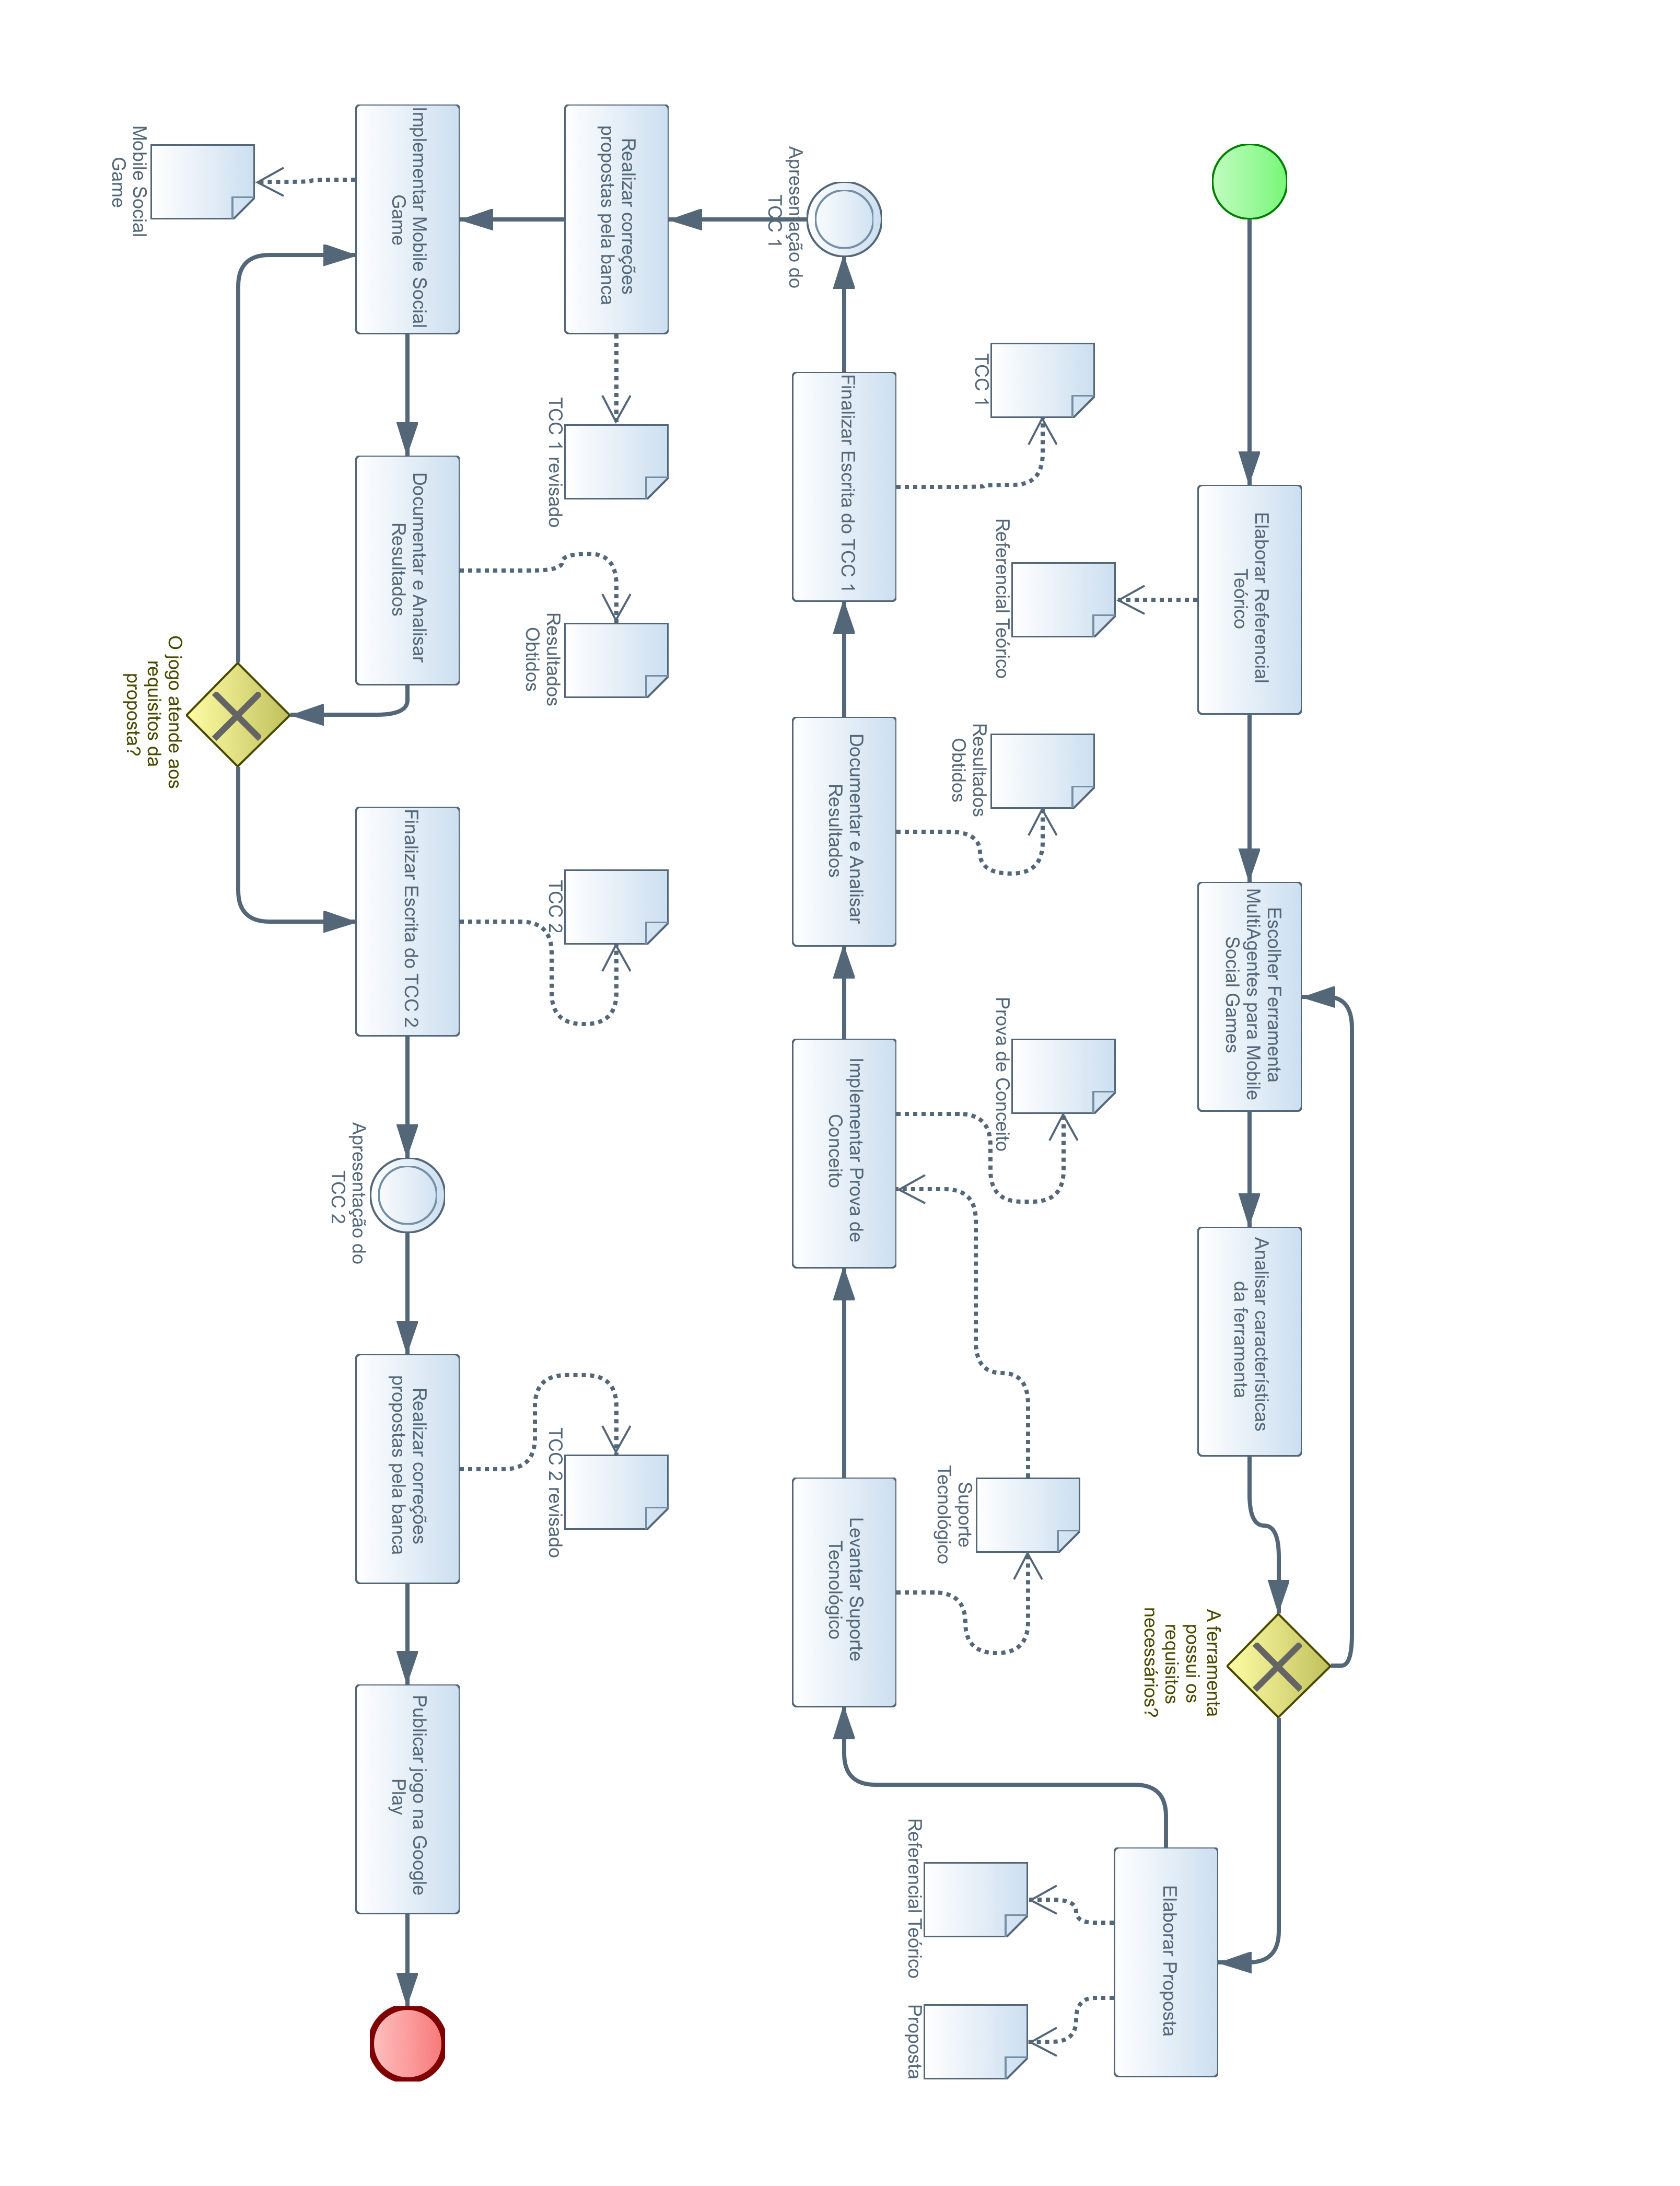
\includegraphics[width=16cm]{figuras/diagram}
  \caption{Processo do TCC}
  \label{figura:diagram}
\end{figure}


\section{Cronograma de Pesquisa}

O cronograma que será seguido para o desenvolvimento desse trabalho pode ser observado na Tabela 1 e Tabela 2. A Tabela 2, referente ao cronograma do TCC 2, é passível de mudanças de acordo com o andamento do trabalho.

%Cronograma 1
\begin{table}[!htbp]
\centering
\resizebox{\textwidth}{!}{%
\begin{tabular}{|l|l|c|c|c|l|}
\hline
\multicolumn{1}{|c|}{\textbf{Atividade}} & \multicolumn{1}{c|}{\textbf{Agosto}} & \textbf{Setembro} & \textbf{Outubro} & \textbf{Novembro} & \textbf{Dezembro} \\ \hline
Levantamento Bibliográfico & \multicolumn{1}{c|}{X} & X & X & \multicolumn{1}{l|}{} &  \\ \hline
Definição do Escopo &  & X & X & \multicolumn{1}{l|}{} &  \\ \hline
Levantamento do Suporte Tecnológico &  & X & X & \multicolumn{1}{l|}{} &  \\ \hline
Implementar Prova de Conceito &  &  & X & X &  \\ \hline
Análise de Resultados &  & \multicolumn{1}{l|}{} & X & X &  \\ \hline
Escrita do TCC 1 &  & \multicolumn{1}{l|}{} & X & X &  \\ \hline
Apresentação do TCC 1 &  & \multicolumn{1}{l|}{} & \multicolumn{1}{l|}{} &  & \multicolumn{1}{c|}{X} \\ \hline
Realizar correções requisitadas pela banca &  & \multicolumn{1}{l|}{} & \multicolumn{1}{l|}{} & \multicolumn{1}{l|}{} & \multicolumn{1}{c|}{X} \\ \hline
\end{tabular}
}
\caption{Cronograma TCC 1}
\label{my-label}
\end{table}


% Cronograma 2
\begin{table}[H]
\centering
\resizebox{\textwidth}{!}{%
\begin{tabular}{|l|l|l|c|c|c|l|}
\hline
\multicolumn{1}{|c|}{\textbf{Atividade}} & \multicolumn{1}{c|}{\textbf{Janeiro}} & \multicolumn{1}{c|}{\textbf{Fevereiro}} & \textbf{Março} & \textbf{Abril} & \multicolumn{1}{l|}{\textbf{Maio}} & \textbf{Junho} \\ \hline
Implementar o Mobile Social Game & \multicolumn{1}{c|}{X} & \multicolumn{1}{c|}{X} & X & X & \multicolumn{1}{l|}{} &  \\ \hline
Documentar e Analisar Resultados &  &  &  & X & X &  \\ \hline
Escrita do TCC 2 &  &  &  & X & X &  \\ \hline
Apresentação do TCC 2 &  &  & \multicolumn{1}{l|}{} &  &  & \multicolumn{1}{c|}{X} \\ \hline
Realizar correções requisitadas pela banca &  &  & \multicolumn{1}{l|}{} & \multicolumn{1}{l|}{} &  & \multicolumn{1}{c|}{X} \\ \hline
\end{tabular}
}
\caption{Cronograma TCC 2}
\label{my-label}
\end{table}


\section{Prova de Conceito}

TODO

\section{Considerações Finais do Capítulo}

TODO
